\begin{problem}
  Consider the differential equation
  \begin{align}\label{diffeq}
    y'' - y = -x,\quad  0<x<1 \quad y(0) = y(1) = 0
  \end{align}
  as in Example 15.12 on page 502.
  Use the basis $\{\phi_j(x)\} = \{x^j(1-x)^j\}$, as in section 15.5.1, to
  compute approximations to the exact solution using the finite-element method.

  Provide relative errors at the points 0.25, 0.50, and 0.75 of the approximations
  using the first $n=2,3,4$ basis functions. Plot
  the corresponding approximations $y_2$, $y_3$, $y_4$, and the exact solution
  $y$. Then find the first value of $j$ for which the relative error at all
  three points is less than 0.5\%.
\end{problem}

\begin{proof}
  The differential equation presented in the problem is a second order linear
  differential equation. It is easily shown that the homogeneous solution is
  given by $y_h(x) = c_1 e^{-x} + c_2e^{x}$ and that a particular solution is
  given by $y_p(x) = x$. Thus the general solution is $y(x) = c_1 e^{-x} + c_2e^{x} + x$.
  Using the boundary conditions, we see that the exact solution is
  \begin{align}\label{exact}
    y(x) = \frac{e^{x}e}{1-e^2} -\frac{e^{-x}e}{1-e^2} + x
  \end{align}

  We now wish to approximate the exact solution $y(x)$.
  Note that the exact solution to the differential equation \eqref{diffeq} is
  a continuous function. This fact combined with the fact that $\{\phi_j(x)\}$
  form a basis of the function space shows that the continuous function $y(x)$
  can be approximated with a linear combination of the basis functions.
  Therefore, we wish to find an approximation $y_n(x)$ to the exact solution
  $y(x)$ where
  \begin{align}\label{finite_approximation}
    y_n(x) = \sum_{j=1}^n a_j \phi_j(x).
  \end{align}
  Note that our basis functions $\{\phi_j(x)\}$ satisfy the boundary
  conditions, i.e.\ $\phi_j(0) = \phi_j(1) = 0$ so that $y_n(x)$ also satisfies the
  boundary conditions.

  Corollary 15.2 suggests that if
  \[
    \int_0^1 (y_n'' - y_n + x)\phi_i(x) dx = 0 \quad \text{for $i=1,\dots,n$}
  \]
  then $y_n'' - y_n + x = 0$, i.e\ $y_n(x)$ satisfies the differential
  equation \eqref{diffeq}. If $y_n(x)$ satisfies the
  differential equation and the boundary conditions, then we know that $y_n(x)$
  approximates the exact solution $y(x)$.

  Therefore, we choose the coefficients $a_j$ such that they satisfy the system of
  equations
  \begin{align}\label{first_system}
    \sum_{j=1}^n a_j \int_0^1 \phi_j''(x)\phi_i(x) - \phi_j(x)\phi_i(x) dx = -\int_0^1 x \phi_i(x) dx \quad \text{for $i=1,\dots,n$}.
  \end{align}

  The above system unnecessarily uses the second derivative of the basis
  functions. We can rewrite the coefficients of the above system to use only
  the first derivative of the basis functions. To see this,
  note that we can rewrite the differential equation \eqref{diffeq} in the form
  \begin{align}\label{alternate_diffeq}
    (p(x)y')' + q(x)y' + r(x)y = f(x)
  \end{align}
  by choosing $p(x) = 1$, $q(x) = 0$, $r(x) = -1$, and $f(x) = -x$. With this form of the
  differential equation we would require the approximation \eqref{finite_approximation}
  to satisfy the following equations
  \[
    \int_0^1 ((p(x)y_n')' + r(x)y_n)\phi_i(x) dx = \int_0^1f(x)\phi_i(x)dx \quad \text{for $i=1,\dots,n$}.
  \]
  Making use of the fact that the basis functions are 0 on the boundary we see that
  \begin{align*}
    \int_0^1(p(x)y_n')'\phi_i(x) dx
    &= \phi_i(x)p(x)y_n'\rvert_0^1 - \int_0^1 p(x)y_n'\phi_i'(x) dx \\
    &= - \int_0^1 p(x)y_n'\phi_i'(x) dx.
  \end{align*}
  With this and the definitions of the functions $p(x)$, $r(x)$, and $f(x)$,
  the system of equations \eqref{first_system} becomes
  \begin{align}\label{system_imp}
    \sum_{j=1}^n a_j \int_0^1 -\phi_j'(x)\phi_i'(x) - \phi_j(x)\phi_i(x) dx = -\int_0^1 x \phi_i(x) dx \quad \text{for $i=1,\dots,n$}.
  \end{align}

  Finding the solution to the system of equations \eqref{system_imp} identifies
  the coefficients $a_j$ that define our approximation.

  In this instance, we have chosen the basis $\left.\{\phi_j(x)\}\right._{j=1}^n$ where $\phi_j(x) = x^j(1-x)^j$.
  Thus,
  \begin{align*}
    \phi_j'(x)
    &= \left(x^j\right)'(1-x)^j + x^j\left((1-x)^j\right)' \\
    &= jx^{j-1}(1-x)^j -jx^j(1-x)^{j-1}
  \end{align*}
  for $j=1,\dots,n$.

  Using the MATLAB function $\texttt{approximation.m}$, we construct the above
  system of equations and solve them arriving at approximations to the exact
  solution for $n=2,3,4$.
  The tables comparing the exact solution to these approximations at the
  points $x=0.25, 0.50, 0.75$ can be found below.

  \begin{table}[h!]
    \centering
    \bgroup
    \def\arraystretch{1.75}
    \begin{tabular}{| l | c | c | c | c |}
      \hline
      $x$ & $y(x)$ & $y_{2}(x)$ & $|y(x) - y_{2}(x)|$ & \pbox{5cm}{$\frac{100|y(x) - y_{2}(x)|}{|y(x)|}$} \\
      \hline
      0.25 & 3.504760e-02 & 4.266210e-02 & 7.614504e-03 & 2.172618e\phantom{-}01 \\
      0.50 & 5.659056e-02 & 5.659010e-02 &      4.598883e-07 &      8.126590e-04 \\
      0.75 & 5.027579e-02 & 4.266210e-02 & 7.613681e-03 & 1.514383e\phantom{-}01 \\
      \hline
    \end{tabular}
    \egroup
    \caption{Comparison of approximation $y_{2}$ to solution $y$ using basis $\phi_j = x^j(1-x)^j$. All computations are rounded to 6 significant digits.}
  \end{table}

  \begin{table}[h!]
    \centering
    \bgroup
    \def\arraystretch{1.75}
    \begin{tabular}{| l | c | c | c | c |}
      \hline
      $x$ & $y(x)$ & $y_{3}(x)$ & $|y(x) - y_{3}(x)|$ & \pbox{5cm}{$\frac{100|y(x) - y_{3}(x)|}{|y(x)|}$} \\
      \hline
      0.25 & 3.504760e-02 & 4.266169e-02 & 7.614092e-03 & 2.172500e\phantom{-}01 \\
      0.50 & 5.659056e-02 & 5.659056e-02 & 5.029993e-10 & 8.888397e-07 \\
      0.75 & 5.027579e-02 & 4.266169e-02 & 7.614093e-03 & 1.514465e\phantom{-}01 \\
      \hline
    \end{tabular}
    \egroup
    \caption{Comparison of approximation $y_{3}$ to solution $y$ using basis $\phi_j = x^j(1-x)^j$. All computations are rounded to 6 significant digits.}
  \end{table}

  \begin{table}[h!]
    \centering
    \bgroup
    \def\arraystretch{1.75}
    \begin{tabular}{| l | c | c | c | c |}
      \hline
      $x$ & $y(x)$ & $y_{4}(x)$ & $|y(x) - y_{4}(x)|$ & \pbox{5cm}{$\frac{100|y(x) - y_{4}(x)|}{|y(x)|}$} \\
      \hline
      0.25 & 3.504760e-02 & 4.266169e-02 & 7.614093e-03 & 2.172500e\phantom{-}01 \\
      0.50 & 5.659056e-02 & 5.659056e-02 & 3.451059e-13 & 6.098294e-10 \\
      0.75 & 5.027579e-02 & 4.266169e-02 & 7.614092e-03 & 1.514465e\phantom{-}01 \\
      \hline
    \end{tabular}
    \egroup
    \caption{Comparison of approximation $y_{4}$ to solution $y$ using basis $\phi_j = x^j(1-x)^j$. All computations are rounded to 6 significant digits.}
  \end{table}

  We also provide the graphs of these comparisons in Figure \ref{poly_plot}.

  \begin{figure}[h!]
    \begin{center}
      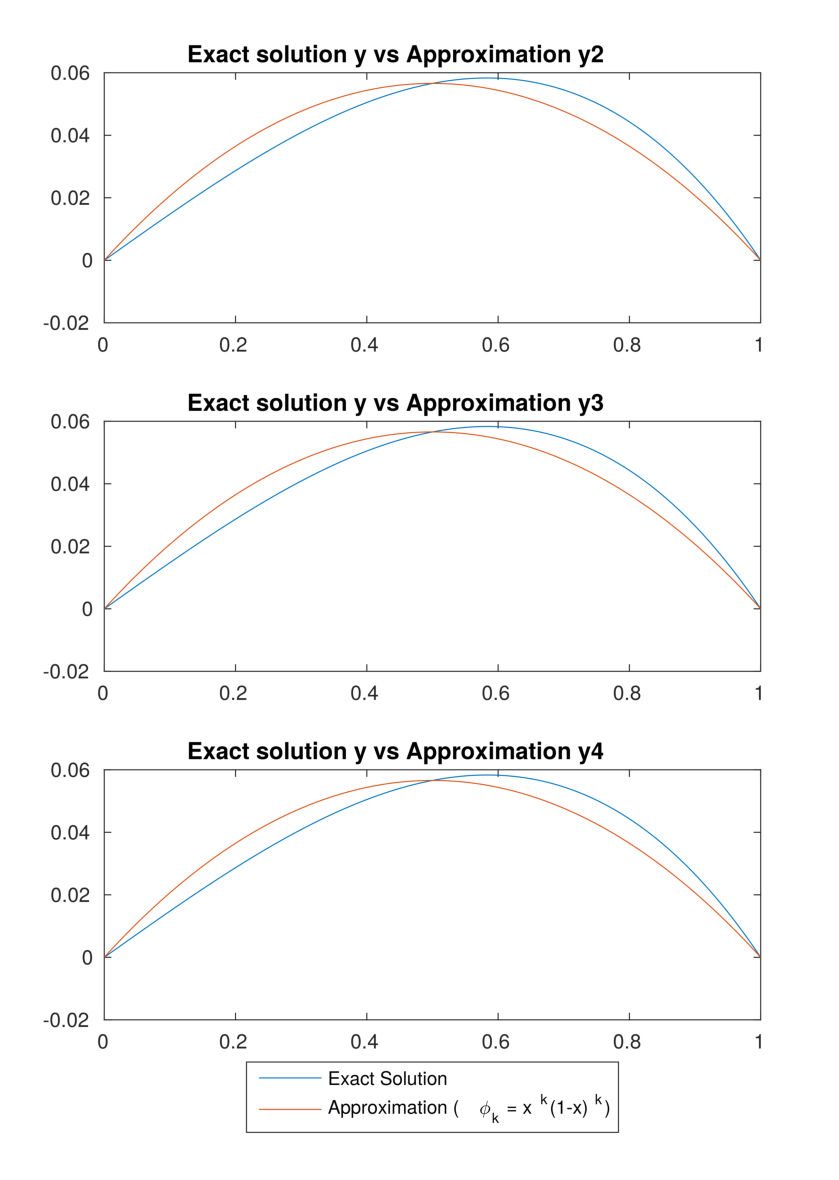
\includegraphics[scale=1.0]{polynomial_basis_comparison}
    \end{center}
    \caption{Plots of exact solution $y$ and approximation $y_n$ over the interval $[0, 1]$
       using basis $\phi_j = x^j(1-x)^j$.}\label{poly_plot}
  \end{figure}

  The first value of $n$ such that the relative error of the approximation at
  each of the points $x_0=0.25, x_1=0.50, x_2=0.75$ is less than 5.0e-01\% is a number larger than 50.
  The relative error percents $r_{x_i}$ for the approximation $y_{50}$ at the above points are given by $r_{x_0}$ = 2.172500e01\%,
  $r_{x_1}$ = 3.576125e-09\%, and $r_{x_2}$ = 1.514465e01\%. You can see that the relative errors at the points $x_0$ and $x_2$ are no
  better than they were for $n=4$. It also appears that these errors do not monotonically decrease towards 0 so that the
  approximation does not practically converge to the exact solution.

  As the coefficient matrix in the system \eqref{system_imp} is dense for this basis,
  we elect not to go any higher than $n=50$ as the computational power needed to solve
  linear systems for dense matrices of large size is higher than
  the author's available hardware can accommodate.

  This suggests that this basis does not give a practical
  approximation to the exact solution at all points of the interval of definition.
  However, as the relative error of the approximation is very small for $n=2$
  at the point $x=0.50$, this suggests that the approximation would be useful
  for neighborhoods with small radius centered at 0.50.

  All programming code used to create the approximations, tables, and graphs
  for this basis can be found here:

  \url{https://github.com/gammadistribution/gradschool/tree/master/MATH635/final/programs/finite_element_approximation}

\end{proof}